\section{Overview Internet of Things and Related Concepts }
\subsection{Internet of Things}
The concept of Internet of Things was first coined by Kevin Ashton, Executive Director of the Auto-ID Center in Massachute Institute of Technology in 1999, and it is described as a world where billions of objects can sense, communicate and share information \cite{madakam2015internet}. Then IoT becomes more popular due to the explosion of mobile devices, ubiquitous communication, cloud computing. However, the definition of ``Internet of Things'' is still ambiguous, and have different facets depending on the perspective. From the view of functionality and identity, IoT is defined as ``Things having identities and virtual personalities operating in smart space using intelligent interfaces to connect and communicate within the social, environmental, and user contexts'' \cite{ray2018survey}. Semantically, the term of Internet of Things is composed of two words ``Internet'' and ``Things''. Following this way, IoT could be defined as ``a worldwide network of interconnected objects uniquely addressable, based on standard communication protocols''~\cite{minerva2015towards}.\\

Similar to its definition, the characteristic of IoT vary from one domain to another. Some of the key characteristics are identified during the research study as follows:

\begin{itemize}
    \item \textbf{Dynamic and Self-adapting}: IoT devices and system must be able to dynamically adapt with the changing contexts or sensed environment. For example, considering a smart building system comprising of a number of temperature devices, these devices can adapt their modes based on whether it is indoor or outdoor. Based on this ability, they can adjust the calibrations to collect data more accurately. In this example, the smart building system is adapting itself with the change of context or environment.
    
    \item \textbf{Self-configuring}: IoT device may have the capability to configure themselves relating connection, software upgrades, etc., while minimal user intervention.  This characteristic allows co-operating a large number of devices to provide specific functionality.
    
    \item \textbf{Interoperable Communication Protocols}: The IoT devices may support multiple connectivity (Wifi, Lora, Sigfox, etc.) to communicate with other devices as well as the cloud infrastructure.
    
    \item \textbf{Unique Identify}: IoT device must be identified by a unique identity (such as an Internet Protocol (IP)\index{IP} address or an Uniform Resource Locator (URL)~\index{URL}). In addition, the IoT system needs to provide intelligent interfaces allowing the end-user to access directly to these devices.
    
    \item \textbf{Integrated into Information Network}: In order to communicate and exchange data, IoT devices are integrated into the information network. In addition, these devices can be dynamically described and discovered in the network by other IoT devices or systems. For example, a weather station can describe its monitoring information to other station in the same information network so that they can communicate and exchange collected data. Such integration could enrich the acquired information because of the data aggregation from several nodes.
    
\end{itemize}

\subsection{Web of Things and Semantic Web of Things}

Recent years, we have been witnessing the explosion of Internet of Things in term of the number and types of IoT devices. Unfortunately, there is no universal application protocol that is compatible with various networking interfaces. Thus, building a single global ecosystem of Things communicating with each other seamlessly is still impossible~\cite{WebofThi19:online}. In other word, the IoT is a collection of ``Silos of Things'' that can not interact with each other. Therefore, to build a global Internet of Things, we need a universal language and protocols supporting the interaction between devices and application regardless of their properties (types, firmware, configuration, etc.). Instead of inventing a dedicated technology, leveraging the widely popular web protocols, standards, and blueprints to make data and services offered by Things more accessible to a larger pool of developer~\cite{guinard2016building}. That is premise behind the adoption of the Web of Things (WoT)~\index{WoT}. The ultimate goal of Web of things is effectively breaking the ``Silos of Things'' also known as ``one device, one protocol, one app'' by applying tools and techniques that are available on the Web technology.\\

In order to archive its goals, WoT is used on the application level to abstract the complexity and variety of lower-level (protocols, firmware, data formats, etc.) by a simple Web model to facilitate the integration of all IoT devices and application. In other words, by hiding the heterogeneity of IoT devices and application behind Web technologies, the WoT allows developers to focus on their applications without considering the technologies behind. In practice, the developers could interact with IoT Things via web browsers and explore the Things as surfing the web. The collected data from Things is visually displayed using Web programming languages such as Hypertext Markup Language (HTML)\index{HTML}, Cascading Style Sheets (CSS)~\index{CSS}, and Javascript.\\ 

In general, the Web of Things facilitates the interaction and exchange of information between different Things and systems powered by Web technologies. However, the exchanged data can be encoded and presented under different formats (envelopes, semantics, and meta-data). For example, the collected data presenting current temperature can be under the plain text, Extensible Markup Language (XML)\index{XML}/Efficient XML Interchange (EXI)\index{EXI}, or JavaScript Object Notation (JSON)\index{JSON} format. The file name can be ``temperature'' or ``temp''. Therefore, it is necessary to build a Semantic Web of Things (SWoT)~\index{SWoT} to ensure a common understanding and format. In other words, SWoT concept is the evolution of the Web on Things with the Semantic technology. The goal of SWoT is to provide comprehensive interoperability that allows not only sharing and reuse of IoT Things but also making IoT data to be universally understandable~\cite{pfisterer2011spitfire}. The summary of evolution from Internet of Things to Web of Things is illustrated in Figure~\ref{fig:c2_evolution_iot_swot}

\begin{figure}[h!] 
 \begin{center} 
 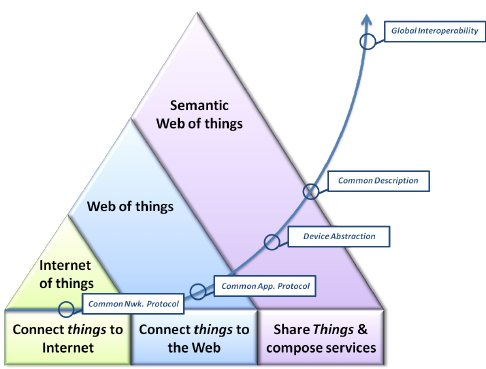
\includegraphics[width=0.72\textwidth]{./Part1/Chapter2/figures/c3_evolution_iot_swot.jpg} 
    \caption{Evolution of the solutions for multicast mobility.~\cite{jara2014semantic}}
     \label{fig:c2_evolution_iot_swot}
  \end{center} 
\end{figure}

\subsection{Massive Internet of Things}

With the explosion of Internet of Things, the number of Things and its connectivity have been growing exponentially. In addition, Things is no longer just send the data to cloud, but also exchange information to each other. As a result, Massive IoT (MIoT)\index{MIoT} is emerging as a new focal point for IoT connectivity technologies referring to the huge volume of constrained IoT devices, which stringently require excellent coverage, cost-effective and low-energy consumption~\cite{Northstream2017}. Among several new connectivity technologies for MIoT, proprietary LPWAN technologies such as Sigfox and LoRa\index{LoRa} have been considering the most potential candidates while cellular-based connectives such as 5G or Narrowband IoT (NB-IoT)\index{NB-IoT} are under developing and testing process \cite{raza2017low}.\\

On the technical level, the IoT devices in Massive Internet of Things context are distributed in a wide area from large manufacturing plants to inside sewer systems where the radio signal is physically challenging. To adapt to such environments, the connectivity technology of Massive IoT is not only wide coverage but also robust. In addition, replacing device battery in large areas is very expensive. This connectivity technology must be low energy consumption to extend the device battery life. Typically, high throughput and latency are not unessential in massive IoT applications, since they more focus on collecting data than controlling.

%%%%%%%%%%%%%%%%%%%%%%%%%%%%%%%%%%%%%%%%%%%%%%%%%%%%%%%%%%%%%%%%%%%%%%%%%%%%%%%%%%%%%%%%%%%%%%%

\section{Fundamentals of IoT}

\subsection{IoT Things}

Similar to Internet of Things definition, deriving a unified definition for the ``Things’’ in IoT is still challenging although it has received the most attention from academic organizations such as National Institute of Standards and Technology (NIST)\index{NIST}, Committed to connecting the world (ITU)\index{ITU}, World Wide Web Consortium (W3C)\index{W3C}, International Energy Research Centre (IERC)\index{IERC}, and Internet Engineering Task Force(IETF)\index{IETF}~\cite{Liu2016}. Institute of Electrical and Electronics Engineers (IEEE)\index{IEEE} simply defined the Things as a physical object that is relevant from a user or application perspective~\cite{minerva2015towards}. However, IERC believes that a Thing can be physical or virtual and identified by unique identity~\cite{smith2012internet}. NIST proposes the Things can be all software, all hardware, or the combination of software and hardware.~\cite{voas2016networks}. \\

Due to the heterogeneity in Things definition, we simplify the Thing could be physical or virtual objects integrated into a network. This object can interact via a unique identity and intelligent interface. For example, a smartphone can be a Thing which is a physical object, able to join networks (WiFi, cellular network), has a unique identity (phone number, IP address) and intelligent interface. A database is also considered as a Thing because it is a virtual object, able to join networks (internet), has a unique identity (URL) and intelligent interface (Web services).

\subsection{IoT Connectivity}

In this section, rather than mentioning all the IoT protocol following existing architecture model like  Open Systems Interconnection model (OSI model) \index{OSI}, we only briefly present some dedicated protocols in IoT and organize them based on their functionality.

\begin{description}
\item[\textbf{Infrastructure}:\\]
    \begin{itemize}
    \item[] 
    \item \textit{6LoWPAN\index{6LoWPAN}: } This is an acronym of IPv6 over Low Power Wireless Personal Area Networks defined by the Internet Engineering Task Force, IETF in their document RFC 6282~\cite{shelby20116lowpan} deriving from the idea that "the Internet Protocol could and should be applied even to the smallest devices,"~\cite{Mulligan:2007:ARC:1278972.1278992}. This protocol uses 2.4 GHz frequency with 250 kbps rate.
    
    \item \textit{uIP\index{uIP}: } The uIP is an open source project licensed under a BDS style license~\cite{adamdunk86:online}. The goal of this project is to create a dedicated TCP/IP stack for 8 or 16 bits micro-controllers. Currently, it is further developed by wide community.
    
    \item \textit{NanoIP\index{NanoIP}: } The concept NanoIP is to optimize all features of Internet to adapt to embedded and small devices, without the overhead of TCP/IP~\cite{shelby2003nanoip}. NanoIP uses two dedicated transport techniques are nanoUPD and nanoTCP. A socket-compatible API is also provided to make sure the protocol similar to original IP protocol.
    
    \item \textit{Time Synchronized Mesh Protocol (TSMP)\index{TSMP}: } TSMP is a communication protocol designed for self-organizing network of wireless devices enabling reliable, low power, secure communication~\cite{pister2008tsmp} 
    
    \end{itemize}

\item[\textbf{Discovery}:\\]
    \begin{itemize}
    \item[] 
    \item \textit{mDNS:\index{mDNS} } The mDNS is used to resolves hostnames to IP addresses within small networks. Except do not include a local name server,  this technology is essentially the same with the unicast Domain Name System (DNS)\index{DNS} in term of programming interfaces, packet formats and operation~\cite{cheshire2013multicast}. 
    
    \item \textit{Physical Web: } The Physical Web aims to discover and interact with nearby devices through a list of URLs being broadcast. That means every smart object in the network needs to broadcast its access URL that any nearby device can receive. 
    
    \item \textit{HyperCat: } HyperCat is an open, lightweight JSON-based hypermedia catalogue format to exploit Thing resources~\cite{HyperCat76:online}. It allows adding a set of semantic annotations to Things resources and makes them discoverable over the web. 
    
    \item \textit{Universal Plug and Play (UPnP)\index{UPnP}: } The UPnP uses Internet and Web protocols to automatically discover new devices to be plugged into a network. These new devices announce their presence to other devices by using a discovery protocol based on Hypertext Transfer Protocol (HTTP)\index{HTTP}~\cite{RFC6970U68:online}. 
    
    
    \end{itemize}

\item[\textbf{Data Protocol}:\\]
    \begin{itemize}
    \item[] 
    \item \textit{Message Queuing Telemetry Transport (MQTT): } MQTT \index{MQTT} is a publish-subscribe based messaging protocol working on the top of TCP/IP protocol. It is useful for connections limited bandwidth~\cite{}. An MQTT system consists of a central messaging server named "message broker" and clients. There are two client types are (1) publisher: clients publish data to broker. (2) Subscriber: Clients receive data from the broker. The responsibility of broker is to forward data from publishers to subscribers. 
    
    \item \textit{Constrained Application Protocol (CoAP): } CoAP \index{CoAP} is an application layer protocol designed for constrained internet devices that are limited in storage, computation power. It is based on RESTful protocol design to simply translate to HTTP for simplified integration, while also meeting specialized requirements such as multicast support, very low overhead, and simplicity~\cite{RFC7252T93:online}. Currently, the major standardization for CoAP is done by IETF and various new functionalities have been added~\cite{colitti2011integrating}. 
    
    \item \textit{Extensible Messaging and Presence Protocol (XMPP): } XMPP \index{XMPP} is a real-time communication protocol based n Extensible Markup Language (XML). It is defined in an open standard managed by IETF. Designed to be extensible, the protocol is also used for the publish-subscribe model in Voice over Internet Protocol (VoIP)~\index{VoIP}, video and IoT applications. 
    
    \item \textit{Advanced Message Queuing Protocol (AMQP): } Similar to XMPP\index{XMPP}, AMQP is an open standard application layer but it is designed for message-oriented middleware. Thereby, its functionalities ensure reliability and security such as message orientation, queuing, routing~\cite{o2007toward}. The authentication and encryption based on Simple Authentication and Security Layer(SASL)\index{SASL} or Transport Layer Security (TLS)\index{SASL}
    
    \item \textit{Lightweight Local Automation Protocol (LLAP): \index{LLAP}} LLAP is a simple short message designed for device to device communication. The key strengths of LLAP are widely compatible and easily understandable by humans~\cite{starksm694:online}.
    
    \end{itemize}
    
\item[\textbf{Communication/Transport layer}:\\]
    \begin{itemize}
    \item[] 
    
    \item \textit{Sigfox: } Sigfox is a radio technology using Ultra Narrow Band (UNB)\index{UNB}. It targets to provide a long range and low energy consumption connectivity for IoT devices. By using UNB, sigfox achieves bandwidth efficiently, low noise levels. However, sigfox is limited in throughput ( only 100bps) and packet size (12 bytes payload)~\cite{}.
    
    \item \textit{Narrow band IoT(NB-IoT): } NB-IOT is a Low Power Wide Area Network (LPWAN)\index{LPWAN} radio technology developed by 3rd Generation Partnership Project (3GPP)\index{3GPP}~\cite{grant20163gpp}. It uses narrowband technology with single frequency 200kHz. Thereby, NB-IoT has limited the bandwidth. In contrast with Sigfox, NB-IoT aims to provide the lost-cost connection in the indoor scenario or dense urban areas in which the connection density is high.
    
    \item \textit{LoRa: } LoRa is a patented digital wireless data communication IoT technology developed by Semtech~\cite{LoRaGate79:online}. It operates over the open license radio frequency bands (169 MHz, 433 MHz, or 868 MHz) enabling long-range transmissions with low power consumption~\cite{LoRaWANR96:online}. The technology of LoRa includes two parts: (1) LoRaPhy: is a communication technology working on physical layer to enable long-range communication link, (2) LoraWan: is an open source communication protocol built upon the LoRaPhy. 
    
    \end{itemize}
    
\end{description}

\subsection{IoT platform}

The IoT platform (also known as IoT middleware) is an intermediate software layer interposed between technique and application layer. Its goal is to abstract the system of hardware complexities under simple interfaces or services. This allows the application developer more focusing on their tasks without concerning the technology behind. In the IoT, such complexities relate to communication because of the considerable heterogeneity in devices, technologies or applications. In such context, the middleware could provide common services or interfaces, which wrap the heterogeneous computing and communication technology of IoT devices. In order to achieve its goals, the middleware needs to fulfill requirements:

\begin{itemize}
    \item \textit{Programming abstraction: } The middleware should provide a simple and common API interface for application developers. This interface is used to separate the developing of application and services with the underlying heterogeneous IoT infrastructures. The style of the programming interface depends on the interface type. For instance, SQL-like languages for data query will be used in descriptive interfaces. \cite{TinyDBAD18:online}.
    
    \item \textit{Interoperable layers: } One of the main goals of middleware is to deal with the heterogeneity in IoT. Thus, the middlewares should equip an interoperable layer to enable the interactions with heterogeneous components in IoT systems including network, syntactic, and semantic perspectives.
    
    \item \textit{Service-based: } A middleware should equip elements to offer high flexibility and reliability services which easily adapt to the frequent changes in middleware functions. 
    
    \item \textit{Adaptive: } A middleware must be able to dynamically adapt and adjust itself with the changes of its context or environments, especially in IoT. 
    
    \item \textit{Context-aware: } Context-aware is the ability to aware the context of users, devices, and environment. This is a key feature to build an adaptive middleware. 
    
    \item \textit{Autonomous: } It means the middleware should be enabled to integrate, communicate and exchange the data with IoT devices without human interactions. To achieve these requirements, there are many technologies including autonomous agents, embedded intelligence, and proactive approaches~\cite{guo2011living}\cite{modukari2005autonomous}
    
\end{itemize}

\subsection{IoT Services }

Because IoT service is an ambiguous term which highly depends on the context, it is hard to provide a concise definition for IoT services. The most common understanding is that ``An IoT-Service is a transaction between service providers and consumers. It triggers a prescribed function to interact (observe, initiate actions, etc.) with the physical world via IoT Things~\cite{barros2012handbook}". Based on this definition, we could classify the IoT services into 2 types:

\begin{itemize}

    \item \textit{Thing-based services: } This kind of services provided by the IoT things allows to connect, obtain and control the Things resources. In powerful IoT things such as smartphone, Raspberry, the services relating Things management and security are also offers. 
    
    \item \textit{Cloud-based services: } These services are provided by the IoT platforms. They may include Things-based services and non-IoT services.
    
\end{itemize}

\subsection{IoT Applications}

The IoT is expected to offer a huge number of applications, which significantly increase our live quality in every aspect: working, living, traveling, etc. In this section, we briefly present the common IoT applications in (1) Transportation domain, (2) Health care domain, (3) Smart environment domain

\begin{itemize}

    \item \textit{Transportation domain: } Vehicles will be more intelligent based on collected information from surrounding context such as traffic status, road quality, nearby objects. The condition of transported goods is also real-time monitored and sent to management system. Based on the information, the managers could optimize their supply chains as well as product quality.
    
    \item \textit{Health care domain: } Wearable devices equipped sensors will help the doctor real-time monitoring patent conditions, particularly on diagnosing potential diseases and problems. Moreover, identifying medication and patient could reduce harmful incidents in the treatment process (such as wrong drug, time, procedure, etc.)
    
    \item \textit{Smart environment: } A smart environment is that make us comfortable and easy thanks to the intelligent of surrounding objects. For instance, sensors and actuators in our office or house could automatically adapt temperature or light relied on the time or our preferences. Moreover, the smart environments also improve the automation in industrial plants based on a large number of sensors and Radio-frequency identification (RFID) \index{RFID} tags. For example, instead manually checking the origin and conditions of products, workers only need to scan RFID tag to gain all necessary information.
    
\end{itemize}

%%%%%%%%%%%%%%%%%%%%%%%%%%%%%%%%%%%%%%%%%%%%%%%%%%%%%%%%%%%%%%%%%%%

\section{IoT Cloud}

\subsection{Cloud Computing}


Following the definition provided by NIST, Cloud computing is a model for enabling ubiquitous, convenient, on-demand network access to shared pool of configurable computing resources (networks, servers, storage, applications, and services)~\cite{mell2011nist}. Over last decade, it strongly impacted the IT industry by offering virtually unlimited storage and computing power at low cost~\cite{spillner2013creating}. Based on these advantages, the IT company could quickly implement and deploy complex IoT solutions. Large companies (Amazon, Google, Facebook, etc.) are typical examples of gaining huge benefits from widely adopting cloud computing. Figure~\ref{fig:c2_cloud_paradigm_overview} presents the main aspects of Cloud including essential characteristics, layered architecture, and standard services mode~\cite{botta2014integration}.

\begin{figure}[h!] 
 \begin{center} 
 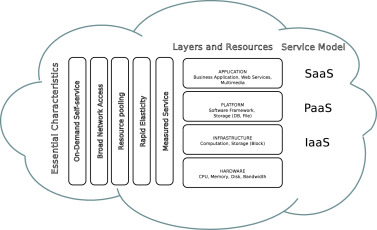
\includegraphics[width=0.5\textwidth]{./Part1/Chapter2/figures/c2_cloud_paradigm_overview.jpg} 
    \caption{Cloud paradigm: An overall view}
     \label{fig:c2_cloud_paradigm_overview}
  \end{center} 
\end{figure}

\par \textbf{A layer model of Cloud computing: } In general, cloud computing architecture is divided in 4 layers:
\begin{itemize}
    \item \textit{The hardware layer: } This layer is used for physical resource management of the cloud such as physical servers, routers, switches, etc. In practice, such layer is deployed in a data center.
    
    \item \textit{The infrastructure layer: } This layer used virtualization technology to partition the physical resources into pools of virtual resources (storage or computing).
    
    \item \textit{The platform layer: } This layer is used to directly deploy applications to virtual resources. It consists of operating systems and application frameworks. 
    
    \item \textit{The application layer: } At the top of architecture, the application layer contains various cloud applications that are better performance, availability and lower operating cost in comparison with traditional applications.
\end{itemize}

\subsection{Cloud-based IoT}

IoT and Cloud computing is disruptive technologies in the Internet era. Fortunately, their characteristics are often complementary in many aspects. In general, IoT is a network of connected things which are limited storage and computing power. This involves concerns about availability, reliability, and performance. In contrast, cloud computing offers unlimited storage and processing power. Thus, a novel IT paradigm is born from the idea about integrating IoT and Cloud Computing to obtain benefits in specific scenarios~\cite{gomes2014future}\cite{alhakbani2014framework}. This paradigm is called CloudIOT. The main benefit of such integration  fall in three categories:

\begin{itemize}

    \item \textit{Communication: } Cloud could provide IoT effective solutions to connect, track and manage the Things (devices, actuators, ....) from anywhere at any time through cloud application or portals. In addition, the high-speed networks facilitate the data collection and control procedure of remote Things~\cite{fox2012architecture}\cite{suciu2013smart}, real-time access to the collected data~\cite{parwekar2011internet}.
    
    \item \textit{Storage: } With the huge number of collected devices, the IOT produce a large amount of non-structured or semi-structured data~\cite{aguzzi2013definition} which also have typical characteristics of big data: volume (data size),  variety (data types), velocity (data frequency). In such scenario, Cloud is the low cost and effective solution thank to large-scale and long-lived storage capabilities. Moreover, after storing on Cloud, the applications can easily access, analyze and visualize from any places. \\
    
    \item \textit{Computation: } The properties of IoT Things are restricted computation power and energy that cannot perform complex operations or data processing. Thus, most of collected IoT data is raw and only processed after conveying to more powerful nodes (gateways, brokers, routers, etc.). Thereby, achieving scalability are very challenging. To deal with these challenges in IoT, Cloud offers unlimited computing power along with on-demand usage model. These capabilities enables IoT data processing on-the-fly, scalability and managing complex events \cite{dash2010survey}\cite{botta2016integration}.
    
\end{itemize}

% \subsection{Cloud-based IoT platform}
% Cloud-based IoT platform is also known as cloud-based IoT middleware is a software implemented on cloud that enables connecting the machines and devices and the acquisition, processing, transformation, and storing sensor data~\cite{inproceedings}

\section{Interoperability in IoT }
\subsection{Interoperability definition}

The distinctive characteristic of IoT is highly heterogeneous in term of devices, technologies, and protocols due to the lack of global standards.
In the IoT context, there is no single definition of the Interoperability term. The most common understanding within the community about this term is that: ``Interoperability is the ability of two systems to interoperate using the same communication protocol''. In a more general view, IEEE defines interoperability as ``the ability of two or more systems or components to exchange information and to use the information that has been exchanged''~\cite{radatz1990ieee}.This ability is separated into 4 levels as illustrated in Fig.~\ref{fig:c2_semantic_interperation_levels}~\cite{morse2004findings}. 

\begin{figure}[h!] 
 \begin{center} 
 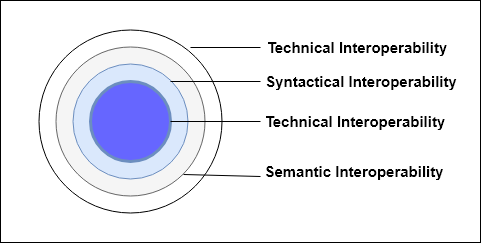
\includegraphics[width=0.6\textwidth]{./Part1/Chapter2/figures/c2_semantic_interperation_levels.png} 
    \caption{The levels of Interoperability}
     \label{fig:c2_semantic_interperation_levels}
  \end{center} 
\end{figure}

\begin{itemize}

    \item \textit{Technical Interoperability: } this is the lowest level in interoperability, usually associated with hardware or software component, system, and platforms enabling machine-to-machine communication. In other words, Technical Interoperability is the ability of IoT components to ``talk'' with each other. Thus, it often focuses on communication protocols and network infrastructures. 
    
    \item \textit{Syntactical Interoperability: } After successfully communicating, the next level of interoperability is highly related to the data formats which are transferred by communication protocols. Syntactical Interoperability is how machines could understand the exchange information.
    
    \item \textit{Semantic Interoperability: } This is usually related to the human interpretation of the content. In other ways, Semantic Interoperability is a common understanding between people about the collected data meaning.
    
    \item \textit{Organizational Interoperability: } This is the highest level of interoperability in which the different organizations could effectively communicate and transfer information regardless of their systems or infrastructures. The organizational interoperability is reached if 3 previous levels are fulfilled.  
\end{itemize}



\subsection{A Interoperability taxonomy}

To understand the IoT interoperability in more detail, we analyze it from the different perspective. As shown in Fig.~\ref{fig:c2_platform_interoperability_overview}, the interoperability is classified into device interoperability, networking interoperability, syntactic interoperability, semantic interoperability, and platform interoperability. 



\begin{figure}[h!] 
 \begin{center} 
 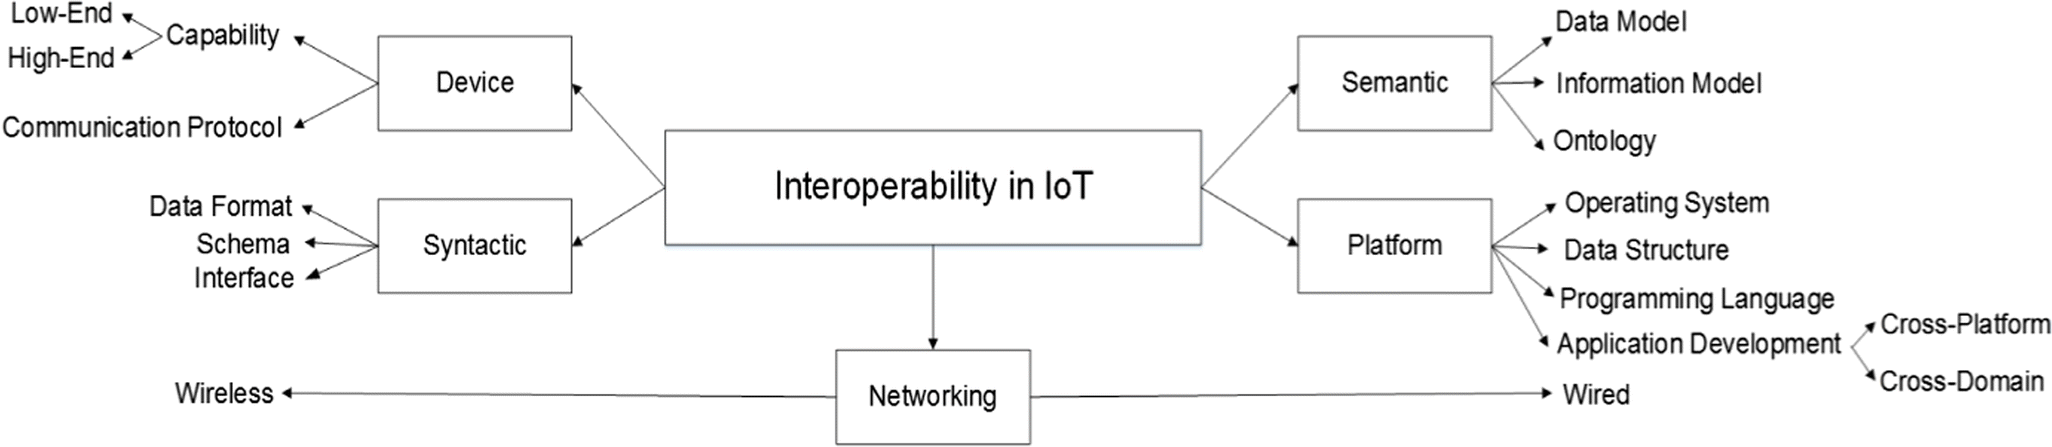
\includegraphics[width=0.9\textwidth]{./Part1/Chapter2/figures/c2_platform_interoperability_overview.png} 
    \caption{The taxonomy of interoperability}
     \label{fig:c2_platform_interoperability_overview}
  \end{center} 
\end{figure}

\begin{itemize}

    \item \textit{Device interoperability: } IoT consists of highly diverse devices which are also known as "smart objects". There are two major device types: (1) the high-end devices have sufficient resources and computational capabilities such as Raspberry Pi, smartphone, etc. (2) the low-end device also known as constrained devices are limited in term of energy, computational power, and communication such as RFID tags, tine sensor, actuator, etc~ \cite{hahm2016operating}. Moreover, many communication protocols have emerged because of the complex requirement of IoT solutions such as Lora, Sigfox, Zigbee, etc. In the missing of a global communication standard, one IoT device is impossible to equip all communication methods. However, in practical, IoT devices have to exchange information with different device types using different communication method. In such case, we need to have interoperability between different types of heterogeneous devices. In summary, device interoperability involves two aspects: (1) the data exchange between heterogeneous IoT devices using heterogeneous communication methods, (2) the ability to integrate new devices into any IoT platform.
    
    \item \textit{Network Interoperability: } Similar to IoT devices, the IoT network services are highly heterogeneous in term of network technology, service, and vendor. Interoperability at network level aims to seamless message exchange through different networks for end-to-end communication. To achieve these goals, IoT network systems should deal with addressing, routing, resource optimization, security and mobility issues~\cite{bello2017network}. 
    
    \item \textit{Syntactical Interoperability: } The data exchanged between heterogeneous IoT systems is usually packed and encode under different formats. Thereby, the message receiver cannot correctly decode and obtain the content of sent messages. Syntactical Interoperability aims to interoperate the format as well as data structure of message exchanged between heterogeneous IoT systems.
    
    \item \textit{Semantic Interoperability: } Following W3C, semantic interoperability is the ability to enable different agents, services, and application to exchange information, data, and knowledge in a meaningful way~\cite{borgia2014internet}. In IoT context, the exchanged data usually use different data models or schemas. This leads to the semantic incompatibility in exchanged information between IoT systems, even if these systems have presented their data and resources to others~\cite{bauer2016semantic}.  
    
    \item \textit{Platform interoperability: } The IoT Platform interoperability is the ability to enable interoperability across IoT platforms in different domains. The Fig.~\ref{fig:c2_platform_interoperability} show the general concept of Platform interoperability that integrates different IoT platforms from different IoT domains to build a common application.It has been emerging because of the diversity of IoT device operation system (OS), data structure, programming languages, and access mechanism for data on cloud. For instance, there are many IoT device OS with different architectures and API such as Contiki, Riot, TinyOS, and OpenWSN. The heterogeneity of IoT platform provider also arises such issues. For example, Apple Homekit supports only Swift programming language, AWS IoT offers an SDK for embedded C and NodeJS. Due to such non-uniformity, application developers need to intensively understand API, information model of each platform. 
\end{itemize}

\begin{figure}[h!] 
 \begin{center} 
 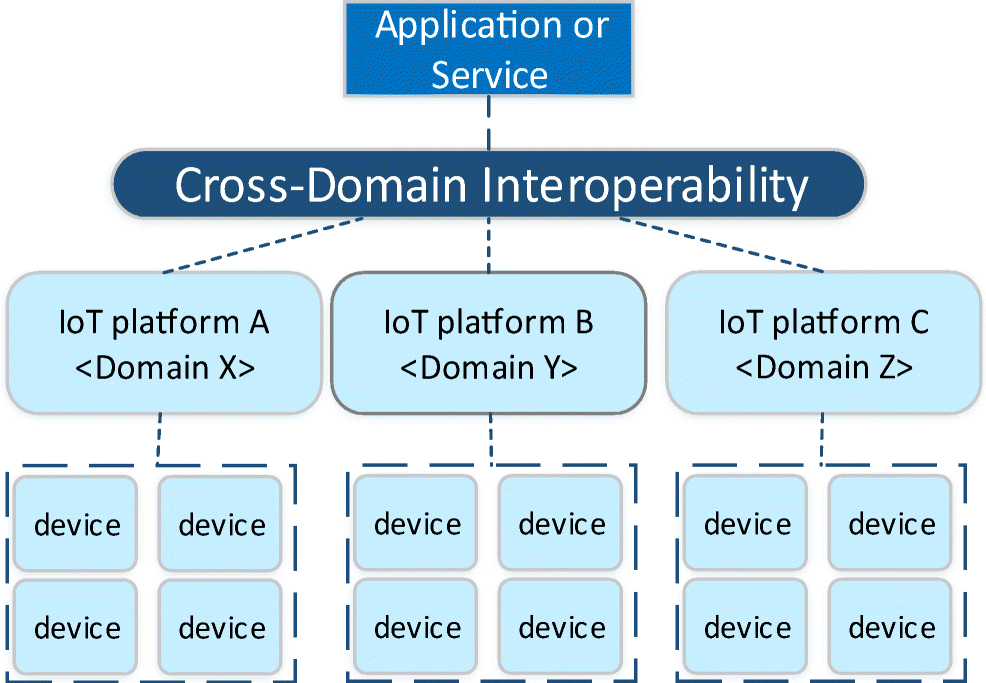
\includegraphics[width=0.6\textwidth]{./Part1/Chapter2/figures/c2_platform_interoperability.png} 
    \caption{The platform interoperability.}
     \label{fig:c2_platform_interoperability}
  \end{center} 
\end{figure}

% \subsection{Interoperability challenges}
%  To achieve comprehensive interoperability, an IoT system needs to be able to interoperate in different layers from device, network, platform to applications. Thereby, there are many challenges to reach this goal. We discuss general issues in interoperability below.
%  \begin{itemize}
%      \item \textit{Low-quality Standards: } In practice, standards are contributed by various individuals or organizations in different backgrounds, purposes. This can cause non-interoperability because (1) Incompleteness: specifications are often missing or partially described the interoperability aspects. (2) redundant options: A standard may include many options which are mostly useless. (3) Poor maintenance: lack of version control and rarely updating the technical changes.
%      \item \textit{Proprietary Technology:} There are many propriety technologies that do not support open APIs or specifications. This strongly affects the universal compatibility of IoT devices.
%      \item \textit{Security: } Enabling interoperability will arise many crucial security issues relating to privacy and secure communication. They involve in establishing the secure communication between IoT devices which have different systems and standards. 
%      \item \textit{Heterogeneous Devices:}
%  \end{itemize}

%%%%%%%%%%%%%%%%%%%%%%%%%%%%%%%%%%%%%%%%%%%%%%%%%%%%%%%%%%%%%%%%%%%%%%%%%%%%%%%%%%%%%%%

\section{Data Outliers in IoT}
\subsection{Definition of data outlier}


In practice, collected data from IoT devices (e.g. sensors, smartphone) is generally unreliable due to the presence of ``dirty-data'' also called data outlier or anomaly. These data outliers are caused by:
\begin{itemize}
    \item \textit{Dropped readings: } The IoT Things are often constrained devices deployed in a restricted environment (e.g. in sewer network, giant factory or plans, etc.). Therefore, the collected data is usually intermittent due to communication errors or scarce resources. 
    \item \textit{Unreliable readings: } Sensor errors, calibration failure among other reasons lead to abnormal data. 
\end{itemize}

The most common definition is that Outliers are outside what is considered as a ``normal state''~\cite{javed2012automated}. Depend on the context of the data, we determine the normal state. For example, 40 celsius degree in summer is normal but it is considered as abnormality if recording in winter.  
In~\cite{branch2013network}, outliers are considered ``events with extremely small probabilities of occurrence''. In another way, they are also seen as ``points in a data set that is highly unlikely to occur given a model of the data.''~\cite{otey2005fast} .

\subsection{Types of outlier}

Based on the definition, outliers are elements that are significantly different from the rest in a dataset. This does not mean all outliers present the errors. In some cases, the outliers contain important information. Based on the context, and carried underlying knowledge, an outlier could be an error or an event~\cite{zhang2010outlier}.

\begin{itemize}

    \item \textit{Erorrs: } An data error involves in a noise measurement or data coming from a faulty IoT device. In practice, the outliers caused by errors significantly outnumber the one caused by events. As such errors reduce the data quality, they need to be correctly identified. Depend on the application, these errors could be eliminated or repaired.
    
    \item \textit{Events: } An event refers to particular phenomena reflected the change of real world (forest fire, watering, etc.). This kind of outlier occurs for a long period of time and create a particular pattern in dataset. However, faulty devices may also create such patterns. Therefore, it is hard to distinguish between event and errors by simply examining dataset statistic. 
    
\end{itemize}

The Outliers caused by errors also named Anomaly is also classified into three  groups\cite{chandola2009anomaly}:

\begin{itemize}

	\item \textbf{Point anomalies}: A single instance of data is anomalous if it is significantly different from the remaining data.
	
	\item \textbf{Contextual anomalies:} The abnormality is context specific. This type of anomaly is common in time-series data. For example 30 Celsius degree during summer is normal but may be abnormal in winter.
	
	\item \textbf{Collective anomalies:} This anomaly type contains a set of consecutive point anomalies to be represented as an abnormal data pattern. This pattern does not comply with the dataset distribution.
	
\end{itemize}

\subsection{Outlier detection}

Outlier detection is a process of discovering the elements that significantly differ from what is considered as normal~\cite{branch2013network}. The final goal is to both eliminate outliers caused by errors and highlight ones caused by events. Outlier detection is an important step in data cleaning process in order to increase data quality. In addition, highlighting outliers caused by events could reveal rare events and patterns underlying in a dataset. The concept of outlier detection is closely related, but much broader than noise removal. It also close to novelty detection which targets to identify the novel pattern in dataset~\cite{chandola2009anomaly}. Outlier detection method can be cataloged into supervised, unsupervised and semi-supervised methods depending on prior information requirements. 

\begin{itemize}

    \item \textit{Unsupervised Outlier detection: } This technique does not require labeled data. The outliers are detected under the assumption that the majority of dataset is normal and abnormal data is only a small proportion. 
    
    \item \textit{Supervised Outlier detection:} This technique requires a training dataset in which normal and abnormal states are labeled. Such dataset is used to train a classifier. 
    
    \item \textit{Semi-supervised Outlier detection: } This technique constructs a classifier model for normal state from clean datasets which are missing abnormal data. Then, this model is used to detect the abnormal data. 
    
\end{itemize}

%%%%%%%%%%%%%%%%%%%%%%%%%%%%%%%%%%%%%%%%%%%%%%%%%%%%%%%%%%%%%%%%%%%%%%%%%%%%%%%%%%%%%%%%%%%%%%

\section{Energy-efficiency in IoT devices}

\subsection{Energy-efficiency definitions}

The Energy-efficiency was first presented as the proportion between total amount of delivered data and total consumed energy~\cite{dietrich2009lifetime}. This means the value of Energy-efficiency is increase if more data is transmitted with less energy consumption. However, Energy-efficiency could be understood in a broader view is ``using less energy to provide the same service''. For instance, a system provides a higher prediction quality while reducing energy consumption could be considered as energy-efficient.\\

The IoT generally consists of small devices with limited power and battery capacity deployed over a wide geographical area. In addition, recharging or replacing battery could be costly or even impossible because IoT devices could be deployed in hostile or restricted environment (e.g. underwater or ground). In many cases, battery life may be required several months or even years. Therefore, the Energy-efficiency has been gaining a vast of attention recently.

\subsection{Device energy consumption}
In order to offer an  Energy-efficiency method, we need to deeply understand the energy consumption model of IoT devices. The authors in~\cite{anastasi2009energy} examined three main sources of power consumption including communication, computation and sensing operation. Although different device types have different energy consumption profile, the overall remarks are:

\begin{itemize}

    \item The communication operations consume much more energy than the computation operation. Therefore, we can trade communication for computation.
    
    \item The radio energy consumption for the reception, transmission, and idle states are the same while the power consumption significantly in the sleep state. Therefore, the radio should be turned off whenever possible.
    
    \item The sensing operations also consume high energy, so it needs to be reduced as much as possible.
    
\end{itemize}

These observations are verified at a sensor platform named TelosB. The authors measured this platform in 95 hours with 100\% duty cycle (no sleep, radio always on, no communication), and 200 hours with a 25\% duty cycle. As the result shown, the radio module is the most energy-consuming component. In addition, we can save energy about ten times in the idle state in comparison with receiving data. 

